\section{Durchführung}

\begin{figure}[H]
    \centering
    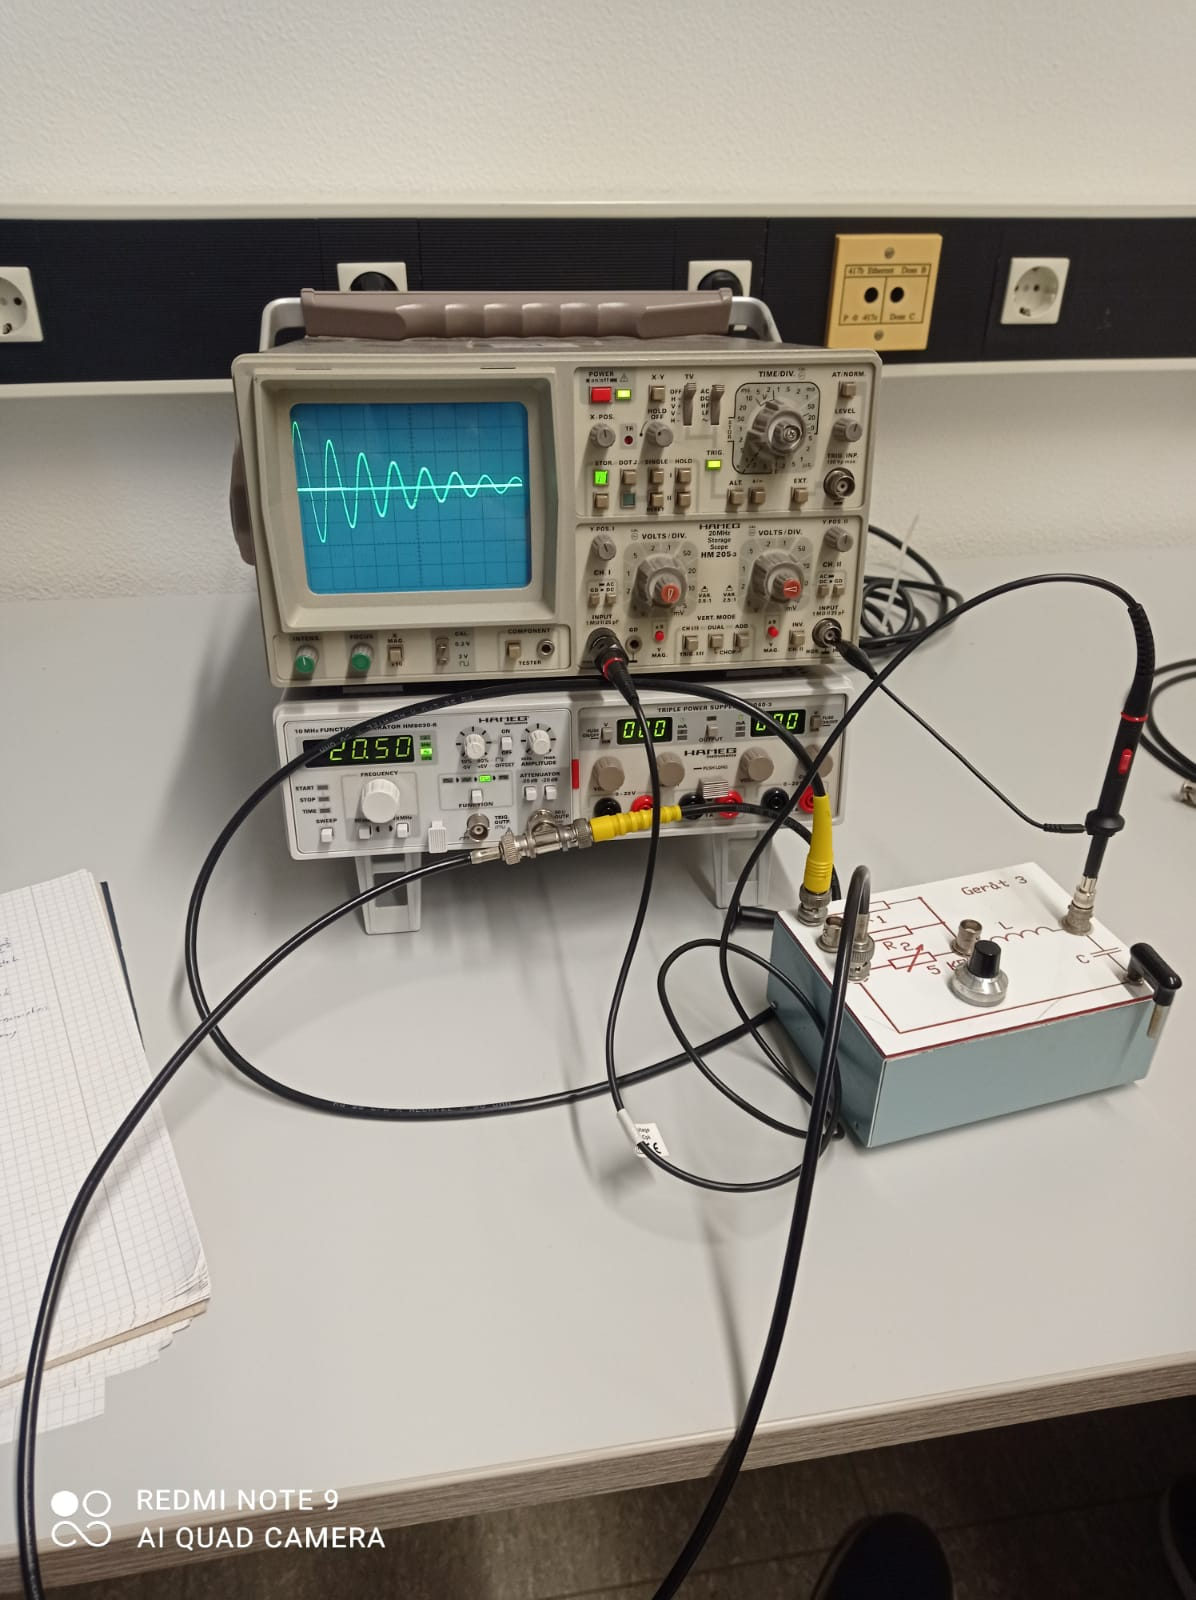
\includegraphics[width=0.6\textwidth]{images/Aufbau.jpeg}
    \caption{Ein Bild des Versuchsaufbau.}
    \label{img:aufb}
\end{figure}

\noindent Der gesamte Versuch wird mit dem in Bild \ref{img:aufb} gezeigten Geräten bearbeitet. Hier sind unten rechts die unterschiedlichen 
Schaltelemte zu sehen. Daneben ist unten der Spannungsgenerator und darauf das Ozsilloskop zum Messen der Schwingungen.

\noindent Als erstes soll die Amplitude der Kondensatorspannung gemessen werden, um über dessen zeitlichen Verlauf den effektiven Dämpfungswiderstand 
zu bestimmen. Dazu wird ein Schaltkreis wie in Abbildung \ref{img:5a} aufgebaut. Der Nadelpulsgenerator und das Oszilloskop werden so eingestellt, dass die 
Amplitude der Kondensatorspannung um einen Faktor zwischen 3 und 8 abnimmt. Für die Messung wird der kleinere Widerstand genutzt.

\begin{figure}[H]
    \centering
    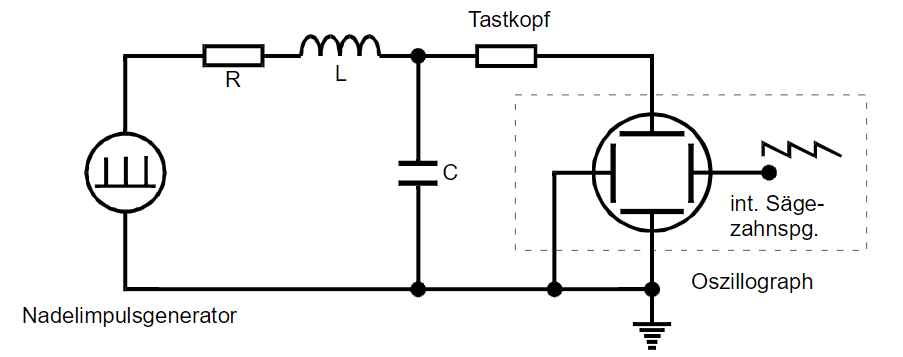
\includegraphics[width=0.6\textwidth]{images/5a.PNG}
    \caption{Aufbau eines RLC-Schwingkreises zur Bestimmung der Kondensatorspannung.}
    \label{img:5a}
\end{figure}

\noindent Als nächstes wird der Widerstand bestimmt bei dem der Spannungsabfall die Form des Aperiodischen Grenzfalls annimmt. Dazu wird der 
Versuchsaufbau wie in Abbildung \ref{img:5b} genutzt. Nun wird der regelbare Widerstand auf sein Maximum gestellt und dann solange reduziert bis
das erste Mal ein Schwingfall eintritt. Der Widerstand wird jetzt langsam so weit erhöt bis die Amplitude der Kondensatorspannung gerade nicht mehr 
unter den Nullpunkt kommt. Dann kann an dem Widerstand $R_{\text{AP}}$ abgelesen werden.

\begin{figure}[H]
    \centering
    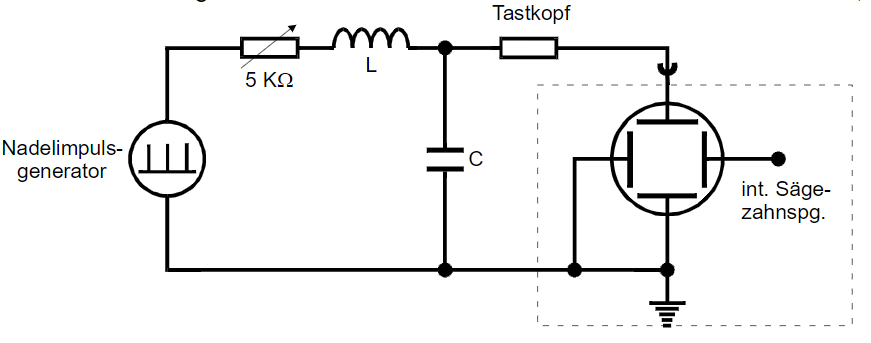
\includegraphics[width=0.6\textwidth]{images/5b.PNG}
    \caption{Aufbau zur Bestimmung von $R_{\text{AP}}$.}
    \label{img:5b}
\end{figure}


\noindent Die dritte Messreihe dient zur Bestimmung der Frequenzabhängigkeit der Kondensatorspannung, um diese Messung durchzuführen wird der 
Aufbau so umgebaut, dass sich die Schaltung wie in Abbidund\ref{img:5c} ergibt. Zunächst wird die Erregerspannung $U$ gemessen. Jetzt kann die 
Frequenz zwischen 100 und $\num{100000}$ variiert werden. In dem Bereich in dem die Kondensatorspannung sein Maximum annimmt, werden die 
meisten Messdaten entnommen.

\begin{figure}[H]
    \centering
    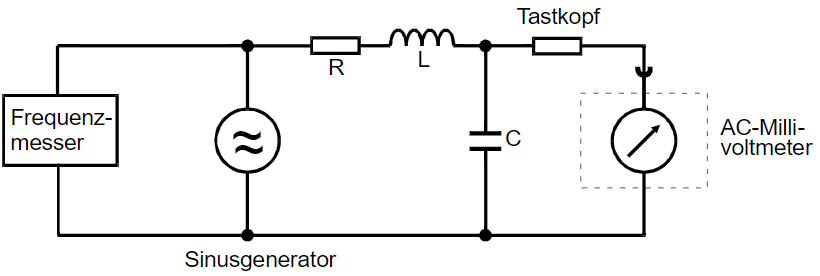
\includegraphics[width=0.6\textwidth]{images/5c.PNG}
    \caption{Aufbau zur Bestimmung der Frequenzabhängigkeit der Kondensatorspannung.}
    \label{img:5c}
\end{figure}

\noindent Im letzten Teil wird die Phasenverschiebung $\phi$ zwischen der Kondensatorspannung $U_{\symup{C}}$ und der Erregerspannung $U$ in 
Abhängigkeit von der anregenden Frequenz bestimmt. Dazu wird ein Aufbau wie in Abbildung \ref{img:5d} aufgebaut. Jetzt werden auf dem Oszilloskop
die Errergerspannung $U$ und die Kondensatorspannung $U_{\symup{C}}$ geplotted. 

\begin{figure}[H]
    \centering
    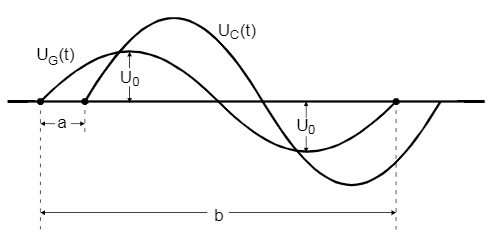
\includegraphics[width=0.6\textwidth]{images/5dplot.PNG}
    \caption{Erregerspannung und Kondensatorspannung geploted.}
    \label{img:5dplot}
\end{figure}

\noindent Dies sollte dann wie in Abbildung \ref{img:5dplot} aussehen, hier wird der Abbstand $a$ zwischen den Nullpunkten und die Periodendauer $b$ 
gemessen, $b$ kann jedoch auch aus der Frequenz berechnet werden.


\begin{figure}[H]
    \centering
    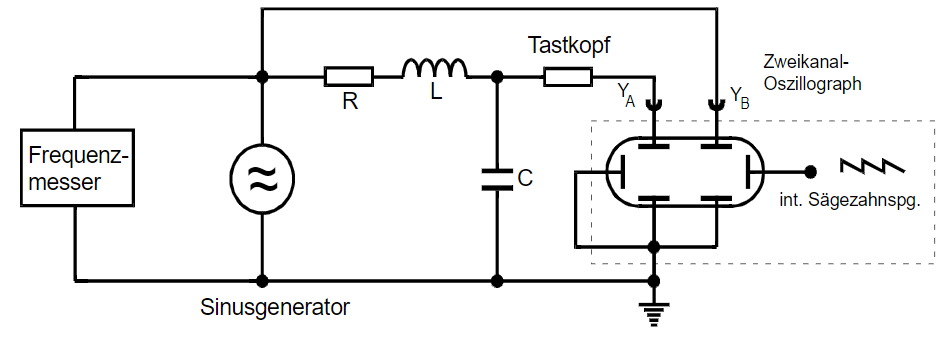
\includegraphics[width=0.6\textwidth]{images/5d.PNG}
    \caption{Aufbau zur Bestimmung der Phasenverschiebung.}
    \label{img:5d}
\end{figure}